\documentclass[11pt]{article}

\usepackage[letterpaper]{geometry}

\usepackage[utf8]{inputenc} % allow utf-8 input
\usepackage{hyperref}       % hyperlinks
\usepackage{url}            % simple URL typesetting
\usepackage{booktabs}       % professional-quality tables
\usepackage{amsfonts}       % blackboard math symbols
\usepackage{nicefrac}       % compact symbols for 1/2, etc.
\usepackage{microtype}      % micro typography
\usepackage{xcolor}         % colors
\usepackage{tikz}           % drawings
\usepackage{pgfplots}       % plots
\usepackage{xfrac}          % better fractions
\usepackage{amsmath,amsthm,amssymb,bm}
\usepackage{comment,todonotes}
\usepackage{graphicx}
\usepackage{natbib}
\usepackage{fancyhdr,sectsty}
\usepackage{fontspec}
\usepackage{caption,subcaption}
\usepackage{minibox}
\usepackage{parskip}
\usepackage[nottoc,numbib]{tocbibind} % Add bibliography to TOC

\newfontfamily\OpenSans[Letters=SmallCaps]{Open Sans}[Scale=MatchLowercase]
\newfontfamily\SourceSerifPro{Source Serif Pro}[Scale=MatchLowercase,Ligatures=TeX]

\bibliographystyle{abbrvnat}

\pgfplotsset{compat=1.18}
\usetikzlibrary{pgfplots.groupplots,positioning,fit,patterns,decorations.pathreplacing}
\usepgfplotslibrary{fillbetween}


% Margins
\topmargin=-4pt
\evensidemargin=0in
\oddsidemargin=0in
\textwidth=6.5in
\textheight=8.5in
\headsep=0.15in

%\pagestyle{fancy}
%\fancyhf{}
%\lhead{Gaurav Manek}
%\rhead{\thepage}
%\rfoot{\thepage}

\title{ On Value Functions in Temporal Difference Learning }
\author{ Gaurav Manek }  
\date{\today}

\newcommand{\E}{\textbf{E}}

\begin{document}

\begin{titlepage}
    {
        \hfill
\includegraphics[width=1.25in,trim=0 0 .125in .25in]{cmu/cmu-wordmark-square-w-on-r.eps}
    }
    \begin{center}{\SourceSerifPro
        \vfill

        {\Huge\OpenSans
            {
                {Value Functions}\\[-.5em]
                \rule{0.25\textwidth}{1pt}
                \raisebox{-.1\baselineskip}{\textit{\Large in}}
                \rule{0.25\textwidth}{1pt}\\[.5em]
                {Temporal Difference Learning}
            }
        }\\


        \vspace{0.25in}

        \textbf{\large Gaurav Manek}\\

        \vfill

        Thesis Proposal

        \textit{In Partial Fulfillment of the Computer Science PhD Program}

        \vspace{0.33in}
        Computer Science Department\\
        School of Computer Science\\
        Carnegie Mellon University\\
        \today

    }\end{center}
\end{titlepage}

\cleardoublepage

~\vfill
\begin{center}
    \begin{minipage}[c]{.7\textwidth}
        \begin{abstract}
            Temporal Difference (TD) learning is used to learn value functions of Markov decision processes (MDPs) using samples following some policy. In Reinforcement Learning (RL), it is necessary to use TD with both function approximation (i.e. neural networks), and off-policy learning. These three conditions are collectively known as the deadly triad because they collectively cause learning to be unstable or diverge. In the literature there are two broad strategies to combat this: regularization and reweighting. Our past work has shown the limitations of regularization, and learned reweighting strategies are well-known to be unstable in practice. We propose a reweighting method based on results from convex optimization with better convergence properties and training performance.
        \end{abstract}
    \end{minipage}
\end{center}

\vfill

\clearpage

\tableofcontents

\clearpage

\section{Introduction}

Temporal Difference (TD) learning is used to learn value functions of Markov decision processes (MDPs) using samples following some policy. In Reinforcement Learning (RL), it is necessary to use TD with both function approximation (i.e. neural networks), and off-policy learning. However, these three ingredients are combined, the learned functions exhibit severe instability and divergence. This was first observed by \citet{tsitsiklis1996analysis}, and is known in the literature as the \emph{deadly triad} \cite[p.~264]{sutton2020reinforcement}. While many variants of TD will provably converge despite the training instability, the quality of the solution at convergence is typically arbitrarily poor \citep{kolter2011fixed}.

There are two separate lines of work in the literature that attempt to resolve this: regularization and Emphatic reweighting.
The former attempts to regularize TD, with $\mathcal L_2$-norm weight regularization (common), $\mathcal L_1$ \citep{mahadevan2014proximal}, convex \citep{yu2017convergence}, and bounds propagation \citep{kumar2020discor}.
The second line started with Emphatic-TD, in which \citet{sutton2016emphatic} note that it is possible to reweight samples obtained off-policy so they appear to be on-policy. Such methods learn the follow-on trace using Monte-Carlo methods (in the original) and/or TD \citep{jiang2021learning,zhang2020provably} or techniques similar to TD \citep{hasselt2021expected}.

Current work on deadly-triad-associated training instability is typically evaluated on three standard examples. However, it is possible to regularize training to mitigate divergence in these, and ridge regularization (RR) is used for that in the literature.
In a paper that is in preparation, we introduce a new counterexample (in Figure~\ref{fig:mdp}) that is resistant to regularization. As expected, vanilla TD-based algorithms converge with arbitrarily poor performance for some off-policy distributions ($\eta=0$ line in Figure~\ref{fig:fixedpoint}), and regularization appears to blunt the asymptote ($\eta > 0$ lines). Part of our contribution is that there is a distribution at which the model never performs better than always guessing zeros (i.e. at the limit of RR $\eta\to\infty$) despite any amount of RR, and hence the model is \emph{vacuous}. This problem persists in any algorithm that converges to the same point as naive TD, which covers a wide swath of the extant literature; we make our analysis concrete by showing how this example forces the error bounds derived by \citet{zhang2021breaking} to permit vacuous solutions.

In the same paper, we show how modern Emphatic algorithms that use TD to learn the reweighting function are vulnerable to the bias introduced by RR. These algorithms (near-universally) assume RR so they converge despite changing policies. We construct a counterexample (Figure~\ref{fig:emphasisplots}) in which the emphasis and value models converge correctly (red circles) when unregularized, but adding regularization causes them to catastrophically diverge (blue circles).

\todo{Mention MVE. }

The focus of our work has now moved on to effectively mitigating this in a manner that is not vulnerable to learning vacuous models or RR-induced bias. We build on the work of \citet{kolter2011fixed}, which derives a condition under which TD is provably stable. Following that work, we have two possible paths. First, we could rewrite the stability criterion so we can compute a closed-form solution for the provably-stable TD update, instead of a nested optimization step. This allows us to reweight updates to be provably stable with only a constant overhead (per iteration) compared to naive TD. Second, we could use Semidefinite Programming (SDP) to compute the reweighting factor for batches of state-transitions. This approach is suitable to larger problems, but we will need to show that the overhead of solving SDPs in the training loop is offset either by better convergence properties or by being able to solve problems that were previously not solvable.

\paragraph{Proposed Thesis Topic:} We propose a novel algorithm to ameliorate the instability from off-policy TD. This algorithm is based on the principles of \cite{kolter2011fixed}, and would work by either (1) computing reweighting factors in a closed-form manner, or (2) by solving an SDP problem for each training minibatch.

\section{Background}

The background to the instability is explained by \citet[p.~264]{sutton2020reinforcement}, and the linear case is analyzed in detail by \citet{kolter2011fixed}. The intuition behind this is that the TD fixed point when sampling on-policy is at the solution of the Bellman equation:
\begin{align}
\Phi \vec w & = R + \gamma\,P\,\Phi \vec w
\intertext{for feature basis $\Phi$, learned weights $\vec w$, reward function $R$, discount factor $\gamma$ and transition matrix $P$. However, when TD updates follow an off-policy distribution $\mu\in \mathbb R^n_0$, the TD solution is instead at the fixed point of the Bellman operator followed by a projection:}
\Phi \vec w & = \Pi_\mu \left( R + \gamma P \Phi \vec w \right)
\intertext{where $\Pi_\mu = \Phi (\Phi^\top D \Phi)^{-1} \Phi^\top D$ projects the Bellman backup onto the columnspace of $\Phi$, reweighted by the diagonal matrix $D = \text{diag}(\mu)$. This yields the closed-form solution:}
\vec w & = A^{-1} \vec b
\intertext{Where $A = \Phi^\top D (I - \gamma P) \Phi$ and $\vec b = \Phi^\top D R$. Under ridge regularization, some small $\eta$ is added to the diagonal of $A$ to ensure that the matrix being inverted is positive definite: }
\vec w & = (A + \eta I)^{-1} \vec b \label{eqn:w}
\end{align}
The intuition behind the training instability is that, for some $\mu$, the matrix $A$ is ill-conditioned or singular, causing the inverse to become arbitrarily large or undefined. This training instability occurs even when the bases $\Phi$ can almost exactly represent the value function.

\label{sec:deadlytriadnaive}
\begin{figure}[!p]
  % !TEX root = proposal.tex
\centering
\begin{subfigure}[b]{0.3\textwidth}
  \centering
  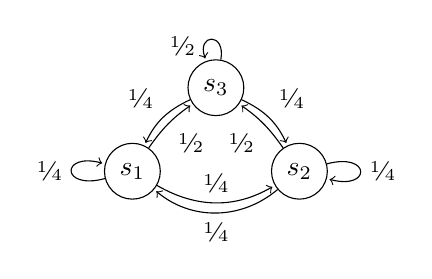
\begin{tikzpicture}[->,shorten >=1pt, node distance={15mm}, main/.style = {draw, circle}] 
    \node[main] (3) {$s_3$}; 
    \node[main] (1) [below left of=3] {$s_1$}; 
    \node[main] (2) [below right of=3]{$s_2$}; 

    \path
    (1) edge[bend left=-30] node[above] {\sfrac 1 4} (2)
        edge[bend right=-10] node[below right] {\sfrac 1 2} (3)
        edge[loop left] node[left] {\sfrac 1 4} (1);

    \path
    (2) edge[bend left=40] node[below] {\sfrac 1 4} (1)
        edge[bend left=-10] node[below left] {\sfrac 1 2} (3)
        edge[loop right] node[right] {\sfrac 1 4} (2);

    \path
    (3) edge[bend left=20] node[above right] {\sfrac 1 4} (2)
        edge[bend right=20] node[above left] {\sfrac 1 4} (1)
        edge[loop above,out=80,in=110,looseness=5] node[left=2mm,pos=0.2] {\sfrac 1 2} (3);

  \end{tikzpicture}
  \caption{Markov Process as a graph.}
  \label{fig:mdp_illustration}

\end{subfigure}
\begin{subfigure}[b]{0.69\textwidth}
  \centering
  \begin{align*}
    \pi = \begin{bmatrix}
      \sfrac 1 4 \\
      \sfrac 1 4 \\
      \sfrac 1 2 \\
    \end{bmatrix}, ~
    \Phi & = \begin{bmatrix}
      1 & 0 \\
      0 & -1 \\
      \sfrac{1}{2} (1.05 + \epsilon) & -\sfrac{1}{2} (1.05 + \epsilon)\\
    \end{bmatrix}, ~
    V = \begin{bmatrix}
      1 \\
      1 \\
      1.05 \\
    \end{bmatrix}
  \end{align*}
  \caption{Stationary distribution $\pi$, Value function basis $\Phi$, True state-values $V$}
  \label{fig:mdp_matrix}
\end{subfigure}

  \caption{Our three-state counter-example MDP. We use this to illustrate how the deadly triad problem persists despite common mitigating strategies. Rewards are set consistent with $V$, and the weights $\vec w$ are trained via TD to minimize $\|\Phi \vec w - V \|$. A small non-zero $\epsilon$ ensures there is some representation error to force the model to approximate the value function: $\|\Phi(\Phi^\top \Phi)^{-1}\Phi^\top V - V \| \leq \epsilon$. }
  \label{fig:mdp}
\end{figure}

\paragraph{Reference Example} There are three examples of this TD runaway common in the literature: the classic Tsitsiklis and Van Roy $(w, 2w)$ example \cite[p.~260]{sutton2020reinforcement}, Kolter's example \cite{kolter2011fixed}, and Baird's counterexample which shows how training instability can exist despite overparameterization \cite{baird1993counterexample}. As explained later, these examples are susceptible to regularization, and so we propose our own novel Markov Reward Process (MRP) to illustrate this effect.

Consider the three-state MRP in Figure~\ref{fig:mdp}, with the stationary distribution $\pi$, value function $V$, and value function basis $\Phi$ as indicated. We arbitrarily choose a discount factor $\gamma = 0.99$, and compute the reward function $R \gets (I-\gamma P)V$. The representation error $\|\Pi_D V - V\| \leq \epsilon$ is small by construction.
Closely following the derivation in \cite{kolter2011fixed}, we show that (when $\eta=0$) there is some off-policy distribution $\mu$ such that the error in the value function learned by TD is unbounded. To do this, we set $\mu = [\sfrac p2, \sfrac p2, 1-p]$ to be a sampling distribution parameterized by $p \in [0..1]$ and find a value of $p$ around which the matrix $A$ is ill-conditioned. Solving $\det(A) = 0$, we obtain:
\begin{align}
  p & = \frac{40400\epsilon^2 + 45240\epsilon + 2961}{40400\epsilon^2 + 84840\epsilon + 4141}\label{eqn:simplep}
\end{align}
Since this solution is in the range $[0, 1]$ for all positive $\epsilon$, there is always some sampling distribution parameter $p$ at which $A$ is ill-conditioned, and hence $A^{-1}$ can be made arbitrarily large by selecting a point close to $p$. We can therefore obtain any error, which completes this introductory example.

We plot the relationship between TD error and $p$ in Figure~\ref{fig:fixedpoint}. The two key features of this are: first, the error is smallest when the sampling distribution $\mu$ is close to the stationary distribution $\pi$ close to $p=0.5$. Second, the error only asymptotically diverges at specific off-policy distributions, notably at about $p=0.715$. It remains low everywhere else.

%%
\begin{figure}[!p]
    \begin{tikzpicture}
    \begin{axis}[
        scale only axis,
        width=\textwidth-10mm,
        height=5cm,
        tick align=outside,
        enlargelimits=false,
        ymode=log,
        mark=none,
        ymax=10,
        xlabel={$p$ in sampling distribution $\mu=[\sfrac p2, \sfrac p2, 1-p]$},
        yticklabels={,,},
        ylabel={TD error},
    ]
    \addplot[color=red,thick] table [x=p, y=err] {fixedpoint/eta_-infty.dat} node[below,pos=0.002] {$\eta=0$};
    \addplot[color=blue] table [x=p, y=err] {fixedpoint/eta_-6.dat} node[above,pos=0.01] {$\eta=10^{-6}$};
    \addplot[color=blue] table [x=p, y=err] {fixedpoint/eta_-4.dat} node[above,pos=0.022] {$\eta=10^{-4}$};
    \addplot[color=blue] table [x=p, y=err] {fixedpoint/eta_-2.dat} node[below,pos=0.1] {$\eta=10^{-2}$};
    \addplot[color=black,thick,dashed] table [x=p, y=err] {fixedpoint/eta_infty.dat} node[above,pos=0.06] {$\eta\to\infty$};
    %\legend{$\eta=0$,$\eta=10^{-6}$,$\eta=10^{-4}$,$\eta=10^{-2}$,$\eta=1$}
    \end{axis}
\end{tikzpicture}

    \caption{We plot TD error against $p$ for the MDP in Figure~\ref{fig:fixedpoint} with $\epsilon=10^{-4}$. This shape is characteristic of TD models in the presence of the deadly triad, including a minima close to $\pi$ ($p=0.5$), and an asymptote at the singular point ($p\approx 0.715$). At different levels of regularization the error function moves between the unregularized case ($\eta=0$) and the limiting case ($\eta\to\infty$).}
    \label{fig:fixedpoint}
\end{figure}
%%

%%%%%%%%%%%%%%%%%%%%%%%%%%%%%%%%%%%%%%%%%%%%%%%%%%%%%%%%%%%%
This is a well-known problem in the literature with many training strategies developed for it, both theoretical and practical. We select some key strategies for discussion here.

\subsection{Ridge Regularization}

One classic solution to this problem is to adopt some sort of regularization to avoid unbounded error or divergence. \emph{Ridge regularization} (RR) \cite{tikhonov1943stability} is the most popular regularization strategy by far, which is generally understood to bound the worst-case error in exchange for biasing the model and potentially increasing the error everywhere else. RR works by penalizing the $\mathcal L_2$-norm of model weights, which limits the scale of the predicted values and the model output. When used to evaluate the deadly triad on three common examples \cite[pg.260]{kolter2011fixed,baird1993counterexample,sutton2020reinforcement}, RR appears to be able to effectively mitigate the worst of the divergence. Consequently, it has become an essential assumption made by many RL algorithms \cite{diddigi2019convergent,mahadevan2014proximal,sutton2009fast,yu2017convergence,zhang2020provably,zhang2021breaking} and is viewed in the literature as a routine and innocuous assumption. Our previous work \citep{manek2022pitfalls} challenges that assumption by introducing counterexamples that shows that training instability is \emph{not} solved by the use of RR.

\paragraph{RR admits vacuous models} Instead of using asymptotic error as a measure of divergence, we define a \emph{vacuous model} as one that, for all $\eta$, never performs better than the limiting error at $\eta\to\infty$. (At the limit $\eta\to\infty$, all model weights are zero and so is the model output.) Intuitively, a vacuous model is one that never does better than always predicting zeros.

Even though RR \emph{appears} to mitigate the training instability, it merely hides it. This can be observed in Figure~\ref{fig:fixedpoint}, which illustrates the effect of RR on the error landscape in our three-state MRP. While RR blunts the asymptote, it increases the error everywhere quickly enough that there is some off-policy distribution under which TD learns always learns a vacuous model despite any amount of regularization. In previous work \citep{manek2022pitfalls}, we identified the exact point and proved this.

\paragraph{RR and small-eta divergence}
Further, there is a general assumption in the literature that RR monotonically shrinks the learned weights and model output. While this is true in classification, regression, and other non-bootstrapping contexts this is \emph{not} true in TD. Because TD repeatedly bootstraps values it is possible for small amounts of model bias to be magnified and induce model divergence.
From Equation~\ref{eqn:w}, we can see that RR ensures the matrix $(A + \eta I)$ is positive definite and therefore invertible without blowing up. This is necessary because, under off-policy distributions, it is possible for $A$ to have eigenvalues that are negative or zero. Adding just the right value of $\eta$ can move these negative eigenvalues arbitrarily close to zero, inducing a correspondingly large error.

We emphasize that this is not just an theoretical concern--we can demonstrate this in the neural network case. Using a 9-state variant of our example and a randomly-assigned value function, and we train 100 randomly-initialized models to convergence. We plot the mean and the $10^\text{th}$--$90^\text{th}$ percentile range in Figure~\ref{fig:multilayerperformance} (left), with and without RR. 
Because we are now working with neural networks and not linear models TD is able to learn models without asymptotes. Since we cannot use asymptotic error to diagnose model divergence, we instead assume that models that perform worse than guessing zero have diverged. Figure~\ref{fig:multilayerperformance} plots this threshold ($\|V\|_2$, dashed grey line). We observe that despite regularization our models perform worse than guessing zero under some off-policy distributions, notably in the domain $p\in[0.1, 0.4]$. This shows that training instability from off-policy learning carries over to the neural network case.

We also plot the TD error against the RR parameter $\eta$ at a fixed off-policy distribution (Fig.~\ref{fig:multilayerperformance}, right). We observe that around $\eta\approx 10^{-3}$ the TD Error unexpectedly \emph{increases} before decreasing. The classic intuition of how ridge regularization works is that it monotonically crushes model parameters (and hence predictions) towards zero, but because TD learns by bootstrapping, the same intuition does not carry over.

\begin{figure}
    \centering

\begin{tikzpicture}
    \begin{axis}[
    width=0.5\textwidth,
    height=0.3\textwidth,
    ymin=0.01,
    ymax=10,
    ymode = log,
    xmin=0,
    xmax=1,
    title = {TD Error over Distributions},
    xlabel={Distribution parameter $p$},
    xtick={0,0.2,0.4,0.6,0.8},
    legend style={legend cell align=left, legend pos=south west,nodes={scale=0.75, transform shape}},
    ]
        \addplot[dashed,color=black] table [x=p, y=v0err] {multilayerperf/basic.dat}
            node[below,pos=0.2] {$\|V\|_2$};

        \addplot[color=red,very thick] table [x=p, y=mean] {multilayerperf/dump_3_0.dat};
        \addplot[color=red,very thin,name path=lcb,] table [x=p, y=conf_05] {multilayerperf/dump_3_0.dat};
        \addplot[color=red,very thin,name path=ucb,] table [x=p, y=conf_95] {multilayerperf/dump_3_0.dat};
        \addplot[pattern=crosshatch,pattern color=red!50,area legend] fill between[of=lcb and ucb];

        \addplot[color=blue,very thick] table [x=p, y=mean] {multilayerperf/dump_3_0.001.dat};
        \addplot[color=blue,very thin,name path=lcb,] table [x=p, y=conf_05] {multilayerperf/dump_3_0.001.dat};
        \addplot[color=blue,very thin,name path=ucb,] table [x=p, y=conf_95] {multilayerperf/dump_3_0.001.dat};
        \addplot[blue!15,area legend] fill between[of=lcb and ucb];

        \legend{,,,,unregularized,regularized}
    \end{axis}
\end{tikzpicture}
\begin{tikzpicture}
    \begin{axis}[
    width=0.5\textwidth,
    height=0.3\textwidth,
    ymin=2.0,
    ymax=4.0,
    xmin=0.00001,
    xmax=1,
    title = {TD Error vs $\eta$ at $p=0.31$},
    xlabel={RR parameter $\eta$},
    xmode=log,
    ]
        \addplot[color=blue,very thick] table [x=eta, y=mean] {multilayerperf/etas_p_0.31.dat};
        \addplot[color=blue,very thin,name path=lcb,] table [x=eta, y=conf_05] {multilayerperf/etas_p_0.31.dat};
        \addplot[color=blue,very thin,name path=ucb,] table [x=eta, y=conf_95] {multilayerperf/etas_p_0.31.dat};
        \addplot[blue!15] fill between[of=lcb and ucb];

        \addplot[dashed,color=black] table [x=eta, y=v0err] {multilayerperf/basic.dat};
    \end{axis}
\end{tikzpicture}

    \caption{On the left we present the mean and $10^\text{th}$--$90^\text{th}$ percentile range of 100 randomly-initialized NN models trained to convergence. On the right we present the relationship between error and the RR parameter $\eta$ at a specific off-policy distribution. We annotate both charts with $\|V\|_2$, which corresponds to the error from guessing zeros. }
    \label{fig:multilayerperformance}
  \end{figure}


\subsubsection{In the literature}

To show that relying on RR is a risky decision to make, we further analyzed our three-state MRP example in the context of the algorithm in \emph{Breaking the Deadly Triad} \citep{zhang2021breaking}. In that paper, the authors assume the use of RR to derive bounds on the learned error under off-policy sampling. We are able to show that their bounds are very loose on our example, permitting vacuous models.

Ridge regularization is particularly common when proving that some training method converges despite a changing sampling policy. This is seen in GTD (analyzed in \cite{yu2017convergence}), GTD2 \cite{sutton2009fast}, RO-TD \cite{mahadevan2014proximal}, and COF-PAC \cite{zhang2020provably}. This assumption may also be used to ensure convergence when training with a target network \cite{zhang2021breaking}. Despite the prevalence of ridge regularization, the induced bias from using it is not well studied in the literature. It is sometimes even dismissed as a mere technical assumption, as in \cite{diddigi2019convergent}. A key conclusion of our prior work contradicts that; using ridge regularization for convergence proofs induces bias that may hinder performance.

RR penalizes the $\mathcal L_2$-norm of the learned weights; it is also possible to use $\mathcal L_1$ regularization with a proximal operator/saddle point formulation as in \cite{mahadevan2014proximal}, or any convex regularization term under a fixed target policy \cite{yu2017convergence}. Instead of directly regularizing the weights, COP-TD uses a discounted update \cite{gelada2019off}. DisCor \cite{kumar2020discor} propagates bounds on Q-value estimates to quickly converge TD learning in the face of large bootstrapping error; it is not clear if DisCor can overcome off-policy sampling. A separate primal-dual saddle point method has also been adapted to ridge regularization \cite{du2017stochastic} and is known to converge under deadly triad conditions, error bounds of this convergence are not yet known.


\subsection{Emphatic-TD Style Algorithms}

Emphatic-TD \cite{sutton2016emphatic} fixes the fundamental problem in off-policy TD by reweighing updates so they appear on-policy. The core idea underlying these techniques is to estimate the ``followon trace'' for each state, the (weighted, $\lambda$- and $\gamma-$discounted) probability mass of all states whose value estimates it influences. This trace is then used to estimate the emphasis, which is the reweighting factor for each update. While this family of methods is provably optimal in expectation, it is subject to tremendous variance in theory and practice, especially when the importance is estimated using Monte-Carlo sampling.\footnote{Sutton and Barto's textbook \citeyearpar{sutton2020reinforcement} says about Emphatic-TD that ``it is
nigh impossible to get consistent results in computational experiments.'' (when applied to Baird's example). } 
There is considerable interest in making this more practical, especially by learning the importance and value models simultaneously.

A leading example of this work is COF-PAC \cite{zhang2020provably}, which uses ridge regularized versions of GTD2 \cite{sutton2009fast} to learn an emphasis model while using that model to also learn a value function. The authors describe RR as essential to their method, particularly when the target policy changes during learning. This reliance on RR makes COF-PAC (and most other TD-based Emphatic algorithms) vulnerable to model bias.
We illustrate this with a counterexample in which COF-PAC diverges because of its reliance on RR.
To generate this counterexample, we apply our three-state MRP to COF-PAC, choosing to learn the value function at the off-policy distribution correponding to $p=0.4$. From Figure~\ref{fig:fixedpoint} we can see that $p=0.4$ lies in the stable region of the error landscape, and so regular TD will converge to a reasonable solution; however, we show how COF-PAC diverges.

COF-PAC has two main parts, an emphasis function and a value function. At each TD update, the emphasis function is updated and then used to reweight incoming value functions. A convenient way to conceptualize COF-PAC is to think in terms of the ``effective'' distribution $\upsilon(\eta)$ (that is, the net distribution after correction.) This depends on (1) the sampling distribution ($\mu$ or $p$ in our example), (2) the regularization applied to the emphasis model during learning, and (3) the target distribution to correct to, typically $\pi$. In Figure~\ref{fig:emphimp}, we fix the target distribution as $\pi$ and plot the error between $\upsilon(\eta)$ and the target distribution as a function of the sampling distribution. When $\eta=0$ we see that the effective distribution $\upsilon(0)$ (red) has a global minima at $p=0.4$. This means that, in our example, COF-PAC will resample input sampled at $p=0.4$ so it appears to be on-policy and the value function will converge to a good solution!

However, if the emphasis model is regularized to $\upsilon(2\cdot 10^{-2})$ (blue), then the distribution error is much higher. This is the crux of our counterexample: we are forced to regularize for good convergence guarantees, but regularizing the emphasis model can bias it so the value model diverges. Figure~\ref{fig:emphval} illustrates the divergence: the unregularized emphasis model (red) corresponds to low error in the value function. Regularizing the emphasis model, however, changes the effective distribution of the value model to one in which it diverges (blue). We also show that regularizing the value function separately does not restore performance.

Intuitively, there is a fundamental bootstrapping issue in this situation: we use an emphasis models because the value function may not converge to a good solution under TD, but to use the emphasis model we have to assume it converges to a good solution under TD. As we show in \cite{manek2022pitfalls}, the use of RR is not sufficient to guarantee good behavior.

\begin{figure}
  \centering
\begin{subfigure}[b]{0.47\textwidth}
  \centering
  \label{fig:emp_weight}

  \begin{tikzpicture}
    \begin{axis}[
        scale only axis,
        width=\textwidth-10mm,
        height=4cm,
        tick align=outside,
        enlargelimits=false,
        mark=none,
        ymax=1.5,
        xlabel={distrib. param. $p$},
        ylabel={distrib. err. $\|\upsilon(\eta) - \pi\|$},
        yticklabels={,,},
        ylabel style={yshift = -9pt,},
    ]
    \addplot[color=red,very thick] table [x=p, y=err] {emphasistd/file_2a0.dat} node[below right,pos=0.7] {$\eta=0$};
    \addplot[color=black,dashed] table [x=p, y=err] {emphasistd/file_2a100..dat} node[above,pos=0.85] {$\eta\to\infty$};
    \addplot[color=blue,very thick] table [x=p, y=err] {emphasistd/file_2a0.0002.dat} node[below,pos=0.2] {$\eta=2\cdot 10^{-2}$};
    % Annotation:
    \addplot[color=red,only marks,mark=o,mark size=6pt] coordinates {(0.4,0)};
    \addplot[color=blue,only marks,mark=o,mark size=6pt] coordinates {(0.4,0.6123)};
    \draw[->,black,very thick,shorten >=6pt,shorten <=6pt] (0.4, 0) to [bend right] (0.4, 0.6123);
    \end{axis}
  \end{tikzpicture}
  \caption{distribution is $[\sfrac p2,~\sfrac p2,~(1-p)]$ }
  \label{fig:emphimp}
\end{subfigure}
\begin{subfigure}[b]{0.47\textwidth}
  \centering

  \begin{tikzpicture}
    \begin{axis}[
        scale only axis,
        width=\textwidth-10mm,
        height=4cm,
        tick align=outside,
        enlargelimits=false,
        mark=none,
        ymax=0.005,
        xlabel={distrib. param. $q$},
        ylabel={value err. $\|\Phi_v w_v^* - V\|$},
        yticklabels={,,},
        ylabel style={yshift = -9pt,},
    ]
    \addplot[color=black] table [x=p, y=err] {emphasistd/file_2b0.dat} node[below right,pos=0.7] {$\eta=0$};
    \draw[red,very thick] (0.5, 0.00086458) -- (0.5, 0.00086458|-{rel axis cs:0,0});
    \draw[red,dashed,very thick] (0.5, 0.005) -- (0.5, 0.005|-{rel axis cs:0,0});
    \draw[blue,very thick] (0.12, 0.005) -- (0.12, 0.005|-{rel axis cs:0,0});

    % Annotation:
    \addplot[color=red,only marks,mark=o,mark size=6pt] coordinates {(0.5,0.00086458)};
    \addplot[color=blue,only marks,mark=o,mark size=6pt] coordinates {(0.12,0.005)};
    \draw[->,black,very thick,shorten >=12pt,shorten <=6pt] (0.5, 0.00086458) to [] (0.12, 0.005);
    \end{axis}
  \end{tikzpicture}
  \caption{distribution is $[\sfrac {(1-q)}2,~\sfrac q2,~0.5]$ }
  \label{fig:emphval}
\end{subfigure}

  \caption{Ridge regularization distorts the emphasis model (left), which induces the value function (right) to move to a singularity. Unregularized models are in red, regularized in blue. Ridge regularization can interact with emphasis models to significantly worsen learned value functions. }
  \label{fig:emphasisplots}
\end{figure}


\subsection{Model-Value Expansion}

A completely different approach from those so far is to factor the value function into parts that we can learn without bootstrapping. In unpublished work \cite{manek2021mve} we investigated the use of Model-Value Expansion (MVE) \cite{Feinberg2018ModelBasedVE}.
The key idea behind MVE is that it is possible to ``unroll'' the computation of a value estimate from a particular state by following a learned dynamics and reward function for a few steps before using a learned value function for the residual value. Since the dynamics and reward function are not bootstrapped, they are not susceptible to divergence from off-policy training. Further, by varying the number of steps and discount factor, it is possible to change the degree of bootstrapping. Informally, this is the modern equivalent to interpolating between Monte-Carlo methods and Bootstrapping, an approach that was explored in the classic RL literature.

Since modern RL algorithms like MBPO \cite{janner2019mbpo} already ensemble independently-initialized dynamics models for synthetic data generation, we can leverage these already-learned models to improve our value estimates. Consequently, such ideas have been explored in the literature \cite{lee2021sunrise,Feinberg2018ModelBasedVE,buckman2018steve}, and have been shown to be effective in standard benchmarks, especially those with continuous state- and action-spaces. The trade-off is that these methods generally require greatly increased computation.

Our prior work \cite{manek2021mve} shows that a small change in ensembling technique greatly improves training performance. We illustrate our technique in Figure~\ref{fig:policyvalue}, where the $i^\text{th}$ dynamics model $f_{(i)}$ and reward model $r_{(i)}$ are independently used to unroll the value estimate for $H$ steps, and the residual value is estimated using a separately-trained $Q$-function. In each critic training step, we fuse these $i$ separate value estimates into a single value by using the mean (or minimum), and use that in the Bellman backup update of the Q-function.
\begin{figure}
    \centering
    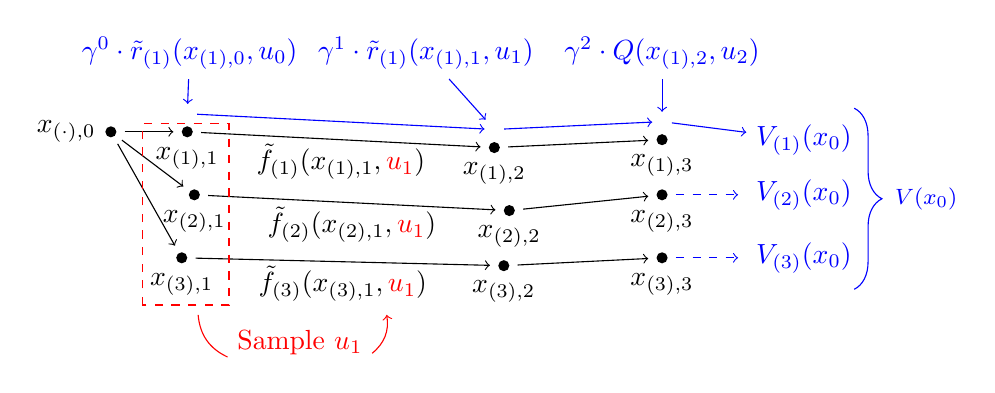
\begin{tikzpicture}[
    line/.style={->,shorten <= 3pt,shorten >= 3pt},
    dot/.style = {circle, fill, minimum size=4pt,inner sep=0pt, outer sep=0pt},
    dot/.default = 6pt  % size of the circle diameter 
    node/.style= {label=below}
]

    \node at (-1,1.0) [dot,label=left:$x_{(\cdot),0}$] (A1) {};

    \node at (-0.03,1.0) [dot,label=below:$x_{(1),1}$] (B1) {};
    \node at (0.06,0.2) [dot,label=below:$x_{(2),1}$] (B2) {};
    \node at (-0.1,-0.6)  [dot,label=below:$x_{(3),1}$] (B3) {};

    \node at (3.87,0.8) [dot,label=below:$x_{(1),2}$] (C1) {};
    \node at (4.06,-0.0) [dot,label=below:$x_{(2),2}$] (C2) {};
    \node at (3.99,-0.7)  [dot,label=below:$x_{(3),2}$] (C3) {};

    \node at (6,0.9) [dot,label=below:$x_{(1),3}$] (D1) {};
    \node at (6,0.2) [dot,label=below:$x_{(2),3}$] (D2) {};
    \node at (6,-0.6)  [dot,label=below:$x_{(3),3}$] (D3) {};

    \draw [line] (A1) -> (B1);
    \draw [line] (A1) -> (B2);
    \draw [line] (A1) -> (B3);

    \draw [line] (B1) -> (C1) node [midway,below=1.8em,label={$\tilde f_{(1)}(x_{(1),1}, {\color{red} u_1})$}] {};
    \draw [line] (B2) -> (C2) node [midway,below=1.8em,label={$\tilde f_{(2)}(x_{(2),1}, {\color{red} u_1})$}] {};
    \draw [line] (B3) -> (C3) node [midway,below=1.8em,label={$\tilde f_{(3)}(x_{(3),1}, {\color{red} u_1})$}] {};

    \draw [line] (C1) -> (D1);
    \draw [line] (C2) -> (D2);
    \draw [line] (C3) -> (D3);
    
    % Action sampling
    \draw[dashed,red] (-.6,-1.2) rectangle +(1.1,2.3);
    \node at (0.0,-1.2)  [] (RL1) {};
    \node at (1.4,-1.4)  [anchor=north,red] (RL2) {Sample $u_1$};
    \node at (2.6,-1.2)  [] (RL3) {};
    \draw [bend right,red] (RL1) edge (RL2);
    \draw [->,bend right,red] (RL2) edge (RL3);

    % Reward
    \node at (0.,2.0) [color=blue] (Q1) {$\gamma^0\cdot\tilde r_{(1)}(x_{(1),0}, u_{0})$};
    \node at (3.0,2.0) [color=blue] (Q2) {$\gamma^1\cdot\tilde r_{(1)}(x_{(1),1}, u_{1})$};
    \node at (6.,2.0) [color=blue] (Q3) {$\gamma^2\cdot Q(x_{(1),2}, u_2)$};
    
    \node [above=1pt of A1] (P0) {};
    \node [above=1pt of B1] (P1) {};
    \node [above=1pt of C1] (P2) {};
    \node [above=1pt of D1] (P3) {};
    \node [right=of D1,color=blue] (PR1) {$V_{(1)}(x_0)$};
    \node [right=of D2,color=blue] (PR2) {$V_{(2)}(x_0)$};
    \node [right=of D3,color=blue] (PR3) {$V_{(3)}(x_0)$};

    % Top
    \draw[->,color=blue] (P3) -> (PR1);
    \draw[->,color=blue] (P2) -> (P3);
    \draw[->,color=blue] (P1) -> (P2);
    \draw[->,color=blue] (Q1) -> (P1);
    \draw[->,color=blue] (Q2) -> (P2);
    \draw[->,color=blue] (Q3) -> (P3);
    
    % Others
    \draw[->,dashed,line,color=blue] (D2) -> (PR2);
    \draw[->,dashed,line,color=blue] (D3) -> (PR3);

    % Max
    \draw [decorate,decoration={brace,amplitude=10pt,mirror,raise=4pt},yshift=0pt,blue] (8.3,-1.0) -- (8.3,1.3) node [blue,midway,xshift=3em] {\footnotesize $V(x_0)$};
\end{tikzpicture}


    \caption{Policy value calculation when $H=2$. Each ensemble member separately unrolls the policy for $H$ steps for MVE and one final step for the terminal value. The action at step $i$ sampled from the joint distribution $\cup_j \pi(x_{(j)},i)$. The value estimate by ensemble member $j$ is $\sum_{a=0}^{H-1} \gamma^a\cdot\tilde r_{(j)}(x_{(j),a}, u_{a}) + \gamma^H Q(\pi(x_{(j)},H))$. The mean (or minimum) of the individual estimates is used as the final value estimate. The exploration temperature is omitted for brevity.}
    \label{fig:policyvalue}
\end{figure}

Through statistical analysis of the learned Q-functions, we show that MVE produces value estimates that are similar to non-MVE estimates from several training steps \emph{in the future}. We conjecture that this mitigates the training delay imposed by the use of target networks. Target networks \cite[]{mnih2015humanlevel} are an absolutely essential part of modern RL algorithms, and they promote training stability by delaying the incorporation of updates into value estimates, preventing an update at some state from influencing the next update to the successor state. Dynamics and reward functions trained in a supervised manner can reduce the delay imposed by the target function while maintaining the important update-independence property.

However, we are not able to show, either in theory or practice, that the use of MVE lessens the propensity of TD to diverge. The mutual dependence between the dynamics models and the learned policy makes this resistant to theoretical analysis, and the natural variance of RL methods makes empirical experimentation cost- and time-prohibitive. As a result we are not pursuing further investigation in this work.


\subsection{Guaranteed-Stable Functions}

%%%%%%%%%%%%%%%%%%%%%%%%%%%%%%%%%%%%%%%%%%%%%%%%%%%%%%%%%%%%
\subsection{Kolter's Non-Expansion Criterion }

In an approach distinct from those proposed so far, \cite{kolter2011fixed} proposes selecting a convex set of ``safe'' distributions and reweighting data so it appears to come from such a distribution. This algorithm, known as TD-DO, is different from Emphatic-TD in that the distribution after reweighting in TD-DO is not necessarily the on-policy distribution, which allows for greater flexibility in training.

These safe distributions are those under which TD updates are guaranteed to be non-expansive. To do this, he writes down this inequality concerning the $D$-norm of the learned value function through one Bellman update, where $D=\text{diag}(\mu)$:
\begin{align}
    \|\Pi_D P\Phi \vec w\|_D & \leq \|\Phi \vec w\|
\intertext{This is true if and only if the matrix $F_D$ is positive semi-definite}
    F_D \equiv & \begin{bmatrix}
        \Phi^\top D \Phi & \Phi^\top D P \Phi \\
        \Phi^\top P^\top D \Phi & \Phi^\top D \Phi
    \end{bmatrix} \succcurlyeq 0 \label{eqn:koltercondmat}
\intertext{This can be written in terms of an expectation over the sampling distribution $\mu$. Let $\mu(s)$ be the PDF of state $s \in \mathcal S$, and the transition distribution $p(s,s') = \mu(s) p(s'|s)$. This condition is equivalent to:}
    \E_{s\sim \mu, s'\sim p(s'|s)} & \left[\begin{bmatrix}
        \phi(s)\phi(s)^\top & \phi(s)\phi(s')^\top \\
        \phi(s')\phi(s)^\top & \phi(s)\phi(s)^\top
    \end{bmatrix}\right] \succcurlyeq 0 \label{eqn:koldercondstate}
\intertext{For convenience, we write down the per-state contribution to this expectation as:}
F(s) = \E_{s'\sim p(s'|s)} & \left[\begin{bmatrix}
    \phi(s)\phi(s)^\top & \phi(s)\phi(s')^\top \\
    \phi(s')\phi(s)^\top & \phi(s)\phi(s)^\top
\end{bmatrix}\right]
\intertext{This allows us to write Equation~\ref*{eqn:koldercondstate}:}
\E_{s\sim \mu} & [F(s)] \succcurlyeq 0
\intertext{In practice this condition does not always hold at $\mu$. We can apply this insight to data by reweighting incoming samples so they are consistent with a different distribution $q$ such that:}
\E_{s~\sim q} & [F(s)] \succcurlyeq 0
\intertext{For input data $(x_1, x_2, \ldots)$, this is the same as finding a set of weights $q_1, q_2, \ldots$ such that:}
\sum_i q_i & \cdot F(x_i) \succcurlyeq 0
\intertext{We also need to constrain our choice of distribution $q$ to ensure the quality of the solution. \citet{kolter2011fixed} achieve this by selecting $q$ that solves this optimization problem}
    \underset{q}{\text{minimize}}~\text{KL}(q||\mu) & \qquad \text{s.t. } ~ E_{s\sim q}[F(s)] \succcurlyeq 0
\end{align}
explicitly optimizing over the distributons using a primal-dual formulation that exploits the structure of the problem.

\clearpage

% \bibliographystyle{plain}
\bibliography{biblio.bib}

\clearpage

\appendix
%\section{Appendix }

\end{document}
